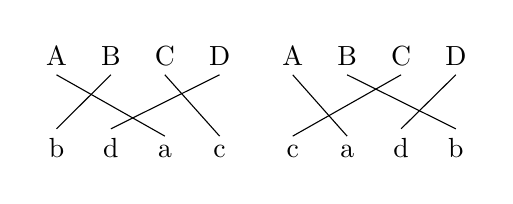
\begin{tikzpicture}[node distance=3cm]
	\usetikzlibrary{matrix}
	\matrix (ex 1) [matrix of nodes,row sep=7mm,column sep=2mm] {
		A & B & C & D \\
		b & d & a & c \\
	};
	\draw (ex 1-1-1.south) -- (ex 1-2-3.north);
	\draw (ex 1-1-2.south) -- (ex 1-2-1.north);
	\draw (ex 1-1-3.south) -- (ex 1-2-4.north);
	\draw (ex 1-1-4.south) -- (ex 1-2-2.north);

	\matrix (ex 2)[matrix of nodes,row sep=7mm,column sep=2mm,right of=ex 1] {
		A & B & C & D \\
		c & a & d & b \\
	};
	\draw (ex 2-1-1.south) -- (ex 2-2-2.north);
	\draw (ex 2-1-2.south) -- (ex 2-2-4.north);
	\draw (ex 2-1-3.south) -- (ex 2-2-1.north);
	\draw (ex 2-1-4.south) -- (ex 2-2-3.north);
\end{tikzpicture}